%Praesentationsmodus
\documentclass[t,aspectratio=169,dvipsnames]{beamer}
%Die Beameroption aspectratio legt das verwendete Seitenverhaeltnis fest
%aspectratio=169	16:9 Seitenverhaeltnis
%aspectratio=1610	16:10 Seitenverhaeltnis
%aspectratio=43		4:3 Seitenverhaeltnis
%Die Beameroption envcountsect nummeriert Umgebungen wie theorem pro section durch.
%Die Beameroption divpsnames wird an das xcolor Paket durchgereicht.

%Handout-Generierung mit Foliennotizen (statt obiger Zeile für den Präsentationsmodus verwenden)
%\documentclass[t,handout,aspectratio=169]{beamer}
%Foliennotizen
%\setbeameroption{show notes}

\usepackage[utf8]{inputenc}

% Deutsch
\usepackage[ngerman]{babel} 
\usepackage{bibgerm}

% Englisch
%\usepackage[english]{babel}

\mode<presentation>
{
\usetheme{HochschuleTrier}
\setbeamercovered{transparent}
}

%\usepackage{mathptmx}
%\usepackage[scaled=0.9]{helvet}
\usepackage{helvet}
\usepackage{courier}
%\usepackage{ae}

\usepackage{hyperref}
\usepackage{tikz}
\usepackage{amsmath}
\usepackage{amsfonts}

\logo{
\includegraphics[height=7.5mm]{HochschuleLogo}}

\usetikzlibrary{calc,positioning}

\usefonttheme[onlymath]{serif}


\usepackage{tikz}
\usepackage{lipsum}
\usepackage{listings}
\lstset
{
	basicstyle=\ttfamily, 
	keywordstyle=\color{blue}\bfseries\ttfamily,
	identifierstyle=\ttfamily, 
	stringstyle=\ttfamily,
	commentstyle=\color{ForestGreen},
	showstringspaces=false,
	framexleftmargin=7mm, 
	breaklines=true,
	tabsize=3,
	showtabs=false,
	frame=single, 
	rulesepcolor=\color{blue},
	numbers=left,
	linewidth=146mm,
	xleftmargin=8mm,
	language={C++},
}


% Stil des Literaturverzeichnisses
\bibliographystyle{geralpha}
%\bibliographystyle{alpha}
%\bibliographystyle{abstract}

%Bitte ausfuellen:
\title{Funktionsprinzipien und Anwendung von Algorithmen zur Pfadplanung}
\subtitle{Eine kurze Einführung mit Beispielen}
\author{Bernardo Cordero, Simon Deutscher, Felix Kalchschmid}							% Autor der Arbeit
\institute{Hochschule Trier}
\date{\today}
\subject{}

%Inhaltsverzeichnisses bis auf subsubsection-Ebene:
%\setcounter{tocdepth}{3}

%Aktivieren, um am Anfang jeder Section ein Inhaltsverzeichnis zur Section anzuzeigen
%\AtBeginSection[]
%{
%\begin{frame}<beamer>
%\frametitle{Agenda}
%\tableofcontents[currentsection,hideothersubsections,sectionstyle=show/hide,subsubsectionstyle=show/show]
%\end{frame}
%}

%Aktivieren, um alles Schritt-fuer-Schritt einzublenden
%\beamerdefaultoverlayspecification{<+->}

\begin{document}

\begin{frame}
\titlepage
\end{frame}

\begin{frame}
\frametitle{Agenda}
\tableofcontents
%\tableofcontents[hideallsubsections] % Subsections ausblenden
%\tableofcontents[pausesections] %Sections Schritt-fuer-Schritt einblenden
\end{frame}

\section{Grundlagen}

\begin{frame}{Was ist Pfadplanung?}{Eine Einführung}
	\begin{columns}[T]
		\begin{column}[T]{0.6\textwidth}
		\begin{itemize}
		\item Pfadplanung ist die Spezifizierung einer Aufgabe in einer Hochsprache, die ein Roboter verstehen und ausführen soll.
		\newline\newline
		\item \textit{Roboter}, \textit{Agent} oder \textit{Player} ist der Nutzer eines Plans, mit dem er Entscheidungen trifft.
	
		\begin{itemize}
		\item Roboter sollen seiner Umgebung verstehen
		\item Roboter haben Bewegungeinschränkungen
		\end{itemize}
		\end{itemize}
		\end{column}
		\begin{column}[T]{0.4\textwidth}
			\begin{figure}
			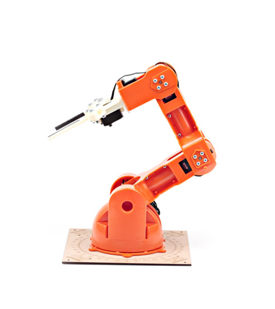
\includegraphics[width=2.5cm]{images/Bild1.png}
			\caption{Testbild in einem figure float}
		\end{figure}
		\end{column}
	\end{columns}
\end{frame}
\subsection{Darstellung des Raums}
\begin{frame}{Darstellung des Raums}{Arbeitsraum und Konfigurationssraum}
	\begin{columns}
		\begin{column}[T]{0.6\textwidth}
			\begin{itemize}
				\item Der Arbeitsraum ist die Welt, in dem der Roboter sich befindet\newline
				\item Konfigurationsraum ist der Raum aller seine Konfigurationen
				\begin{itemize}
					\item Konfiguration ist die Position der Roboter in seiner verständliche Sprache
					\item Hindernisse sind ungültige Konfigurationen
					\item Freier Raum ist die Gruppe von Konfigurationen ohne Kollisionen
					
				\end{itemize}
			\end{itemize}
		\end{column}
		\begin{column}[T]{0.4\textwidth}
			\begin{figure}
				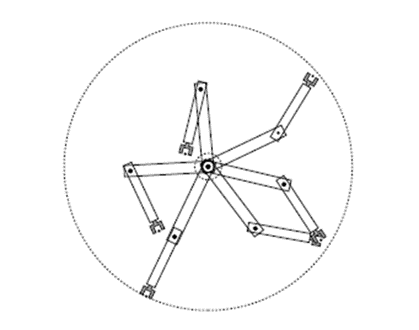
\includegraphics[width=4.5cm]{images/Bild2.png}
				\caption{Testbild in einem figure float} 
			\end{figure}
		\end{column}
	\end{columns}
\end{frame}

\begin{frame}{Darstellung des Raums}{Potentialfeld}
			\begin{itemize}
				\item Punkte in dem Konfigurationsraum bekommen eine Potentialvektor.
				\begin{itemize}
					\item Sie wehren Hindernisse ab
					\item Sie werden vom Ziel angezogen
				\end{itemize}
			\end{itemize}
		
			\begin{figure}
				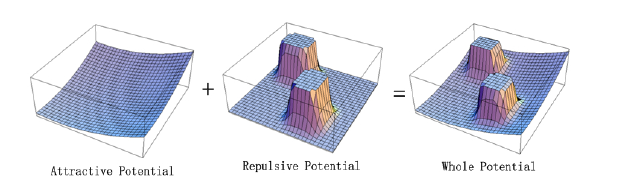
\includegraphics[width=10.5cm]{images/Potential_Field.png}
				\caption{Testbild in einem figure float} 
			\end{figure}
\end{frame}
\begin{frame}{Darstellung des Raums}{Roadmap}
	\begin{columns}
		\begin{column}[T]{0.6\textwidth}
			\begin{itemize}
				\item Die Punkte des Konfigurationsraum verbinden
				\item Bewegung in Roadmap durch:
				\begin{itemize}
					\item Roadmap eintreten
					\item Roadmap durchlaufen
					\item Ziel erreichen
				\end{itemize}
				\item Sichtbarkeitsgraphen sind Roadmaps	
			\end{itemize}
		\end{column}
		\begin{column}[T]{0.4\textwidth}
			\begin{figure}
				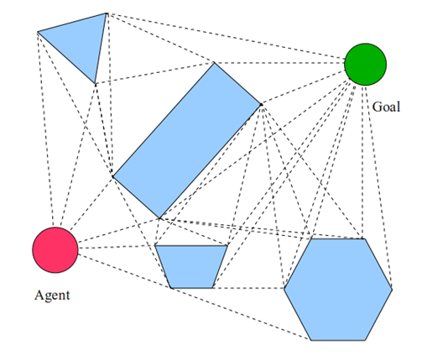
\includegraphics[width=4.5cm]{images/Bild3.png}
				\caption{Testbild in einem figure float} 
			\end{figure}
		\end{column}
	\end{columns}
\end{frame}

\begin{frame}{Darstellung des Raums}{Zelldekomposition}
	\begin{itemize}
		\item Teilung des freies Raums in Zellen
		\begin{itemize}
			\item Verbindungen zwischen anliegenden Zellen speichern
		\end{itemize}
	    \item Zellen enthalten Start- und Endkonfigurationen beim Pfadfindung.
	\end{itemize}
	
	\begin{figure}
		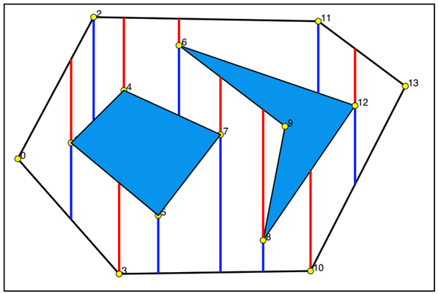
\includegraphics[width=5.0cm]{images/Bild4.png}
		\caption{Testbild in einem figure float} 
	\end{figure}
\end{frame}
\subsection{Graphen}
\begin{frame}{Graphen}{Eine Einführung}
	\begin{itemize}
		\item Graphen sind gut für Pfadfindung
		\item Ein Graph besteht aus Knoten, Kanten und Kosten
		\item Gerichteter Graphen unterscheiden ausgehende und eingehende Kanten
	\end{itemize}
	
	\begin{figure}
		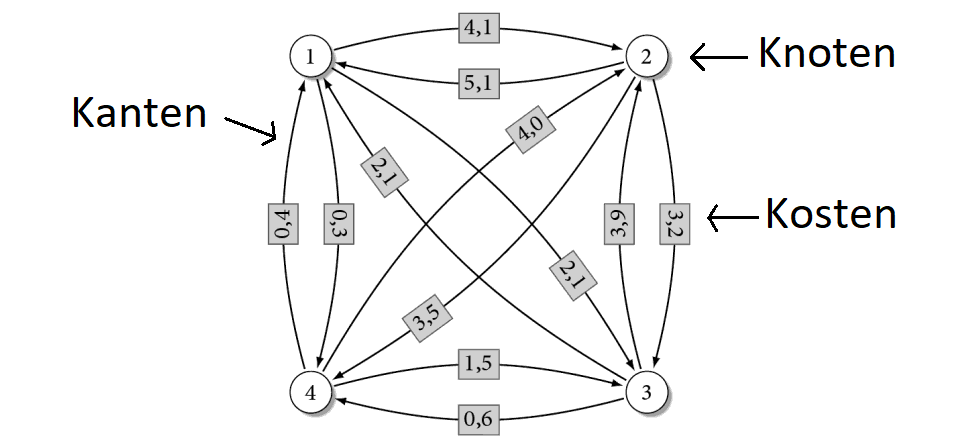
\includegraphics[width=7.0cm]{images/kk_graph_S6.png}
		\caption{Testbild in einem figure float} 
	\end{figure}
\end{frame}

\begin{frame}{Graphen}{Bäume}
	\begin{itemize}
		\item Hierarchische Darstellung von Graphen
		\item Ein Baum hat ein Wurzel
		\item Knoten haben Tiefe: Entfernung von Wurzel
	\end{itemize}
	
	\begin{figure}
		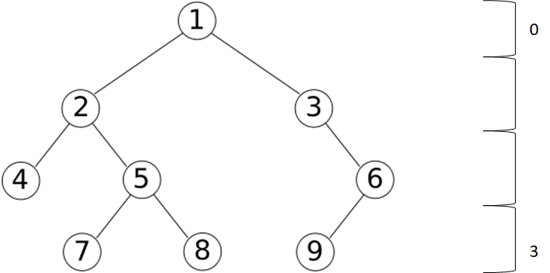
\includegraphics[width=7.0cm]{images/Bild5.png}
		\caption{Testbild in einem figure float} 
	\end{figure}
\end{frame}
\begin{frame}{Graphen}{Navigationsnetze}
	\begin{columns}
		\begin{column}[T]{0.5\textwidth}
			\begin{itemize}
				\item Navigationsnetze definieren der freie Raum als polygonale Bereiche
				\item Verbindungen zwischen Bereiche sind in Navigationsgraph gespeichert
				\item Start und Endkonfigurationen befinden sich in die Bereiche
			\end{itemize}
		\end{column}
		\begin{column}[T]{0.5\textwidth}
			\begin{figure}
				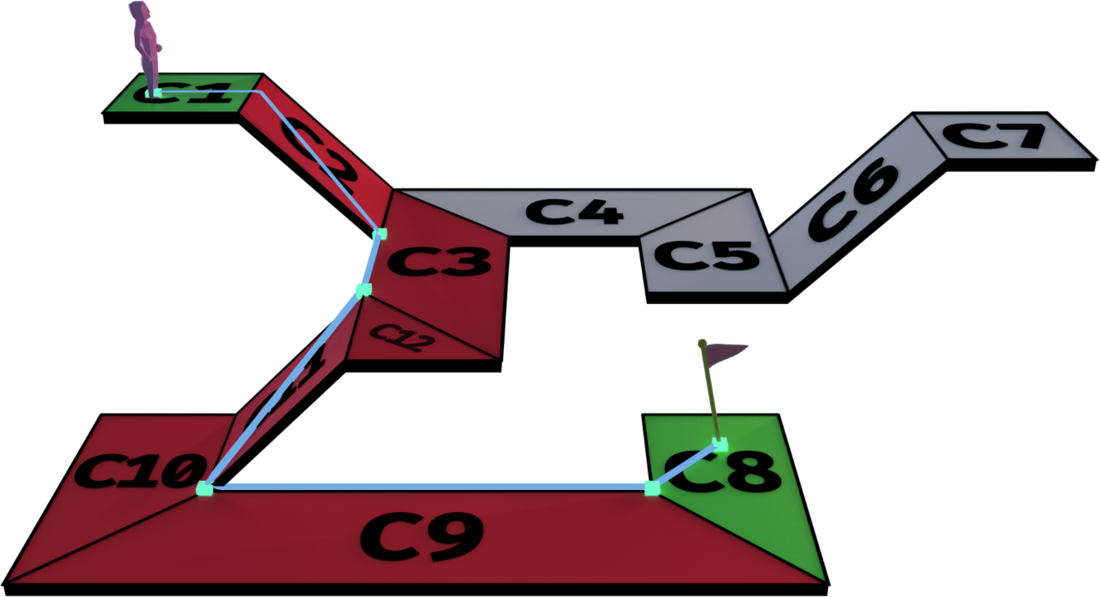
\includegraphics[width=6.5cm]{images/mesh_with_path.png}
				\caption{Testbild in einem figure float} 
			\end{figure}
		\end{column}
	\end{columns}
\end{frame}

\begin{frame}{Graphen}{Rastergraphen}
	\begin{itemize}
		\item Raum in Felder definieren
		\begin{itemize}
			\item Felder können verschieden Formen haben
		\end{itemize} 
		\item Die Felder kennen ihre Nachbarn
	\end{itemize}
	\begin{figure}
		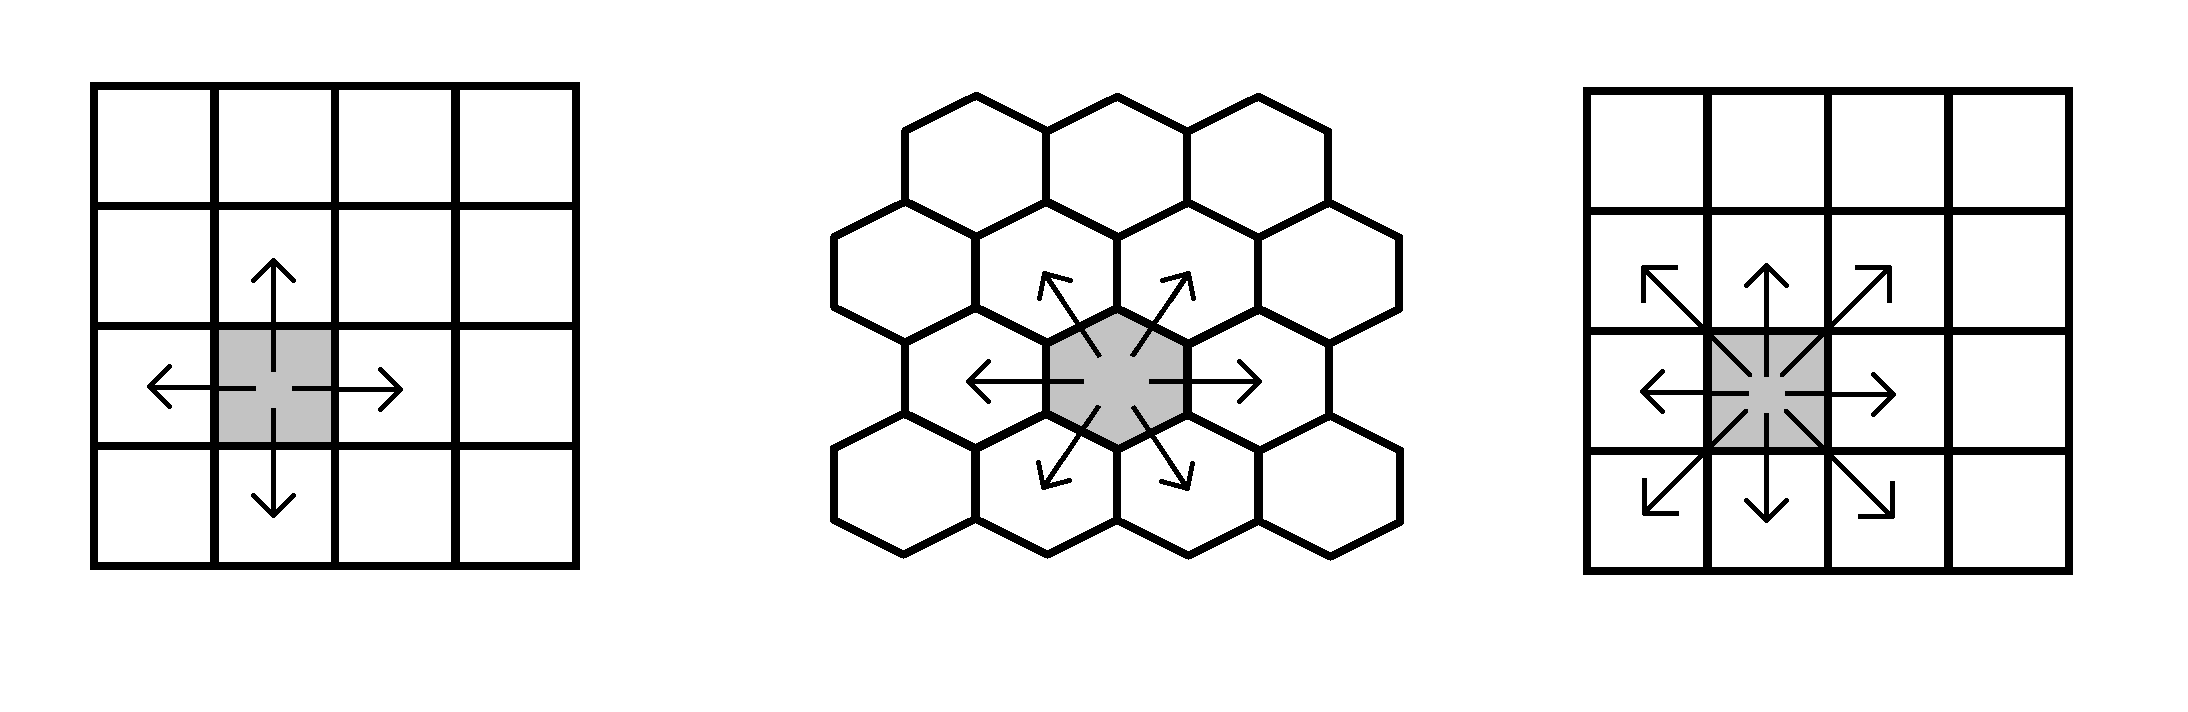
\includegraphics[width=10.0cm]{images/Grid_Tiles.png}
		\caption{Testbild in einem figure float} 
	\end{figure}
\end{frame}

\begin{frame}{Graphen}{Sichtbarkeitsgraphen}
	\begin{columns}
		\begin{column}[T]{0.5\textwidth}
			\begin{itemize}
				\item Roadmap aus sichtbare Punkte bilden
				\item Die Eckpunkte der Hindernisse verbinden
				\item Sensoren nehmen neue Information für den Roboter, um neue  Kanten zu bilden
			\end{itemize}
		\end{column}
		\begin{column}[T]{0.5\textwidth}
			\begin{figure}
				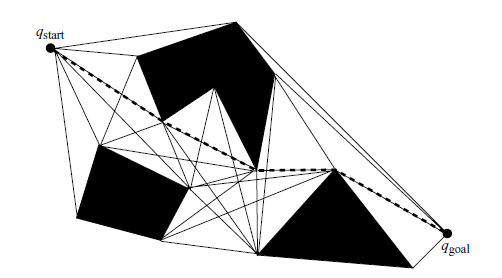
\includegraphics[width=6.5cm]{images/Robot_Motion_Visibility_Graph.png}
				\caption{Testbild in einem figure float} 
			\end{figure}
		\end{column}
	\end{columns}
\end{frame}
\section{Algorithmen}

\begin{frame}{Graphen}{Sichtbarkeitsgraphen}
	\begin{columns}
		\begin{column}[T]{0.5\textwidth}
			\begin{itemize}
				\item Roadmap aus sichtbare Punkte bilden
				\item Die Eckpunkte der Hindernisse verbinden
				\item Sensoren nehmen neue Information für den Roboter, um neue  Kanten zu bilden
			\end{itemize}
		\end{column}
		\begin{column}[T]{0.5\textwidth}
			\begin{figure}
				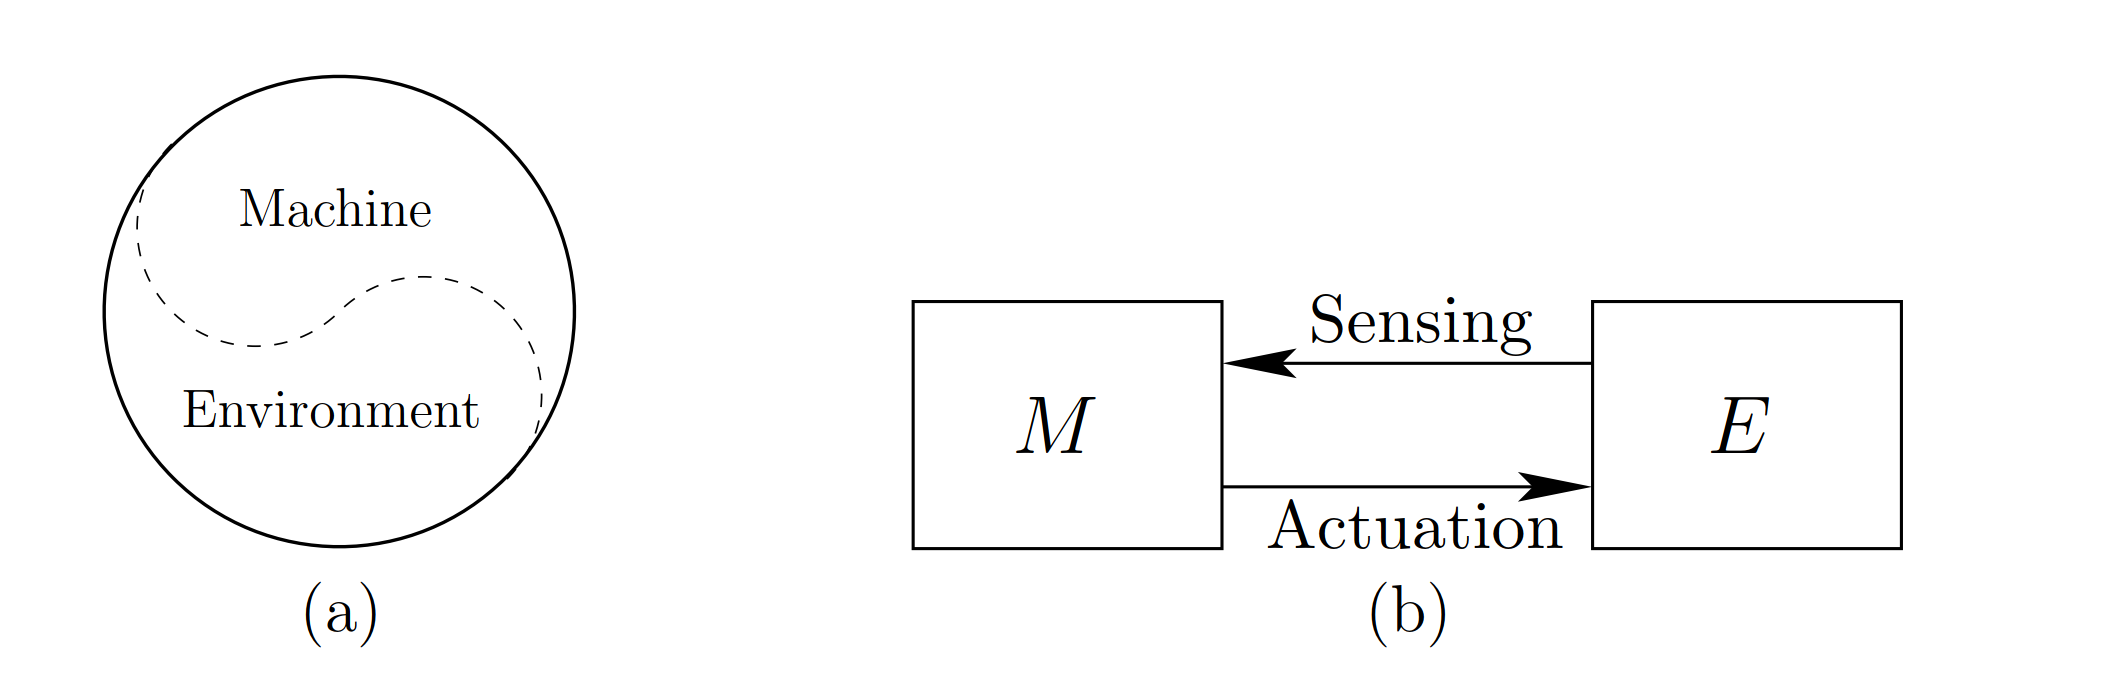
\includegraphics[width=6.5cm]{images/img224.png}
				\caption{Testbild in einem figure float} 
			\end{figure}
		\end{column}
	\end{columns}
\end{frame}
\begin{frame}{Graphen}{Sichtbarkeitsgraphen}
	\begin{columns}
		\begin{column}[T]{0.5\textwidth}
			\begin{itemize}
				\item Roadmap aus sichtbare Punkte bilden
				\item Die Eckpunkte der Hindernisse verbinden
				\item Sensoren nehmen neue Information für den Roboter, um neue  Kanten zu bilden
			\end{itemize}
		\end{column}
		\begin{column}[T]{0.5\textwidth}
			\begin{figure}
				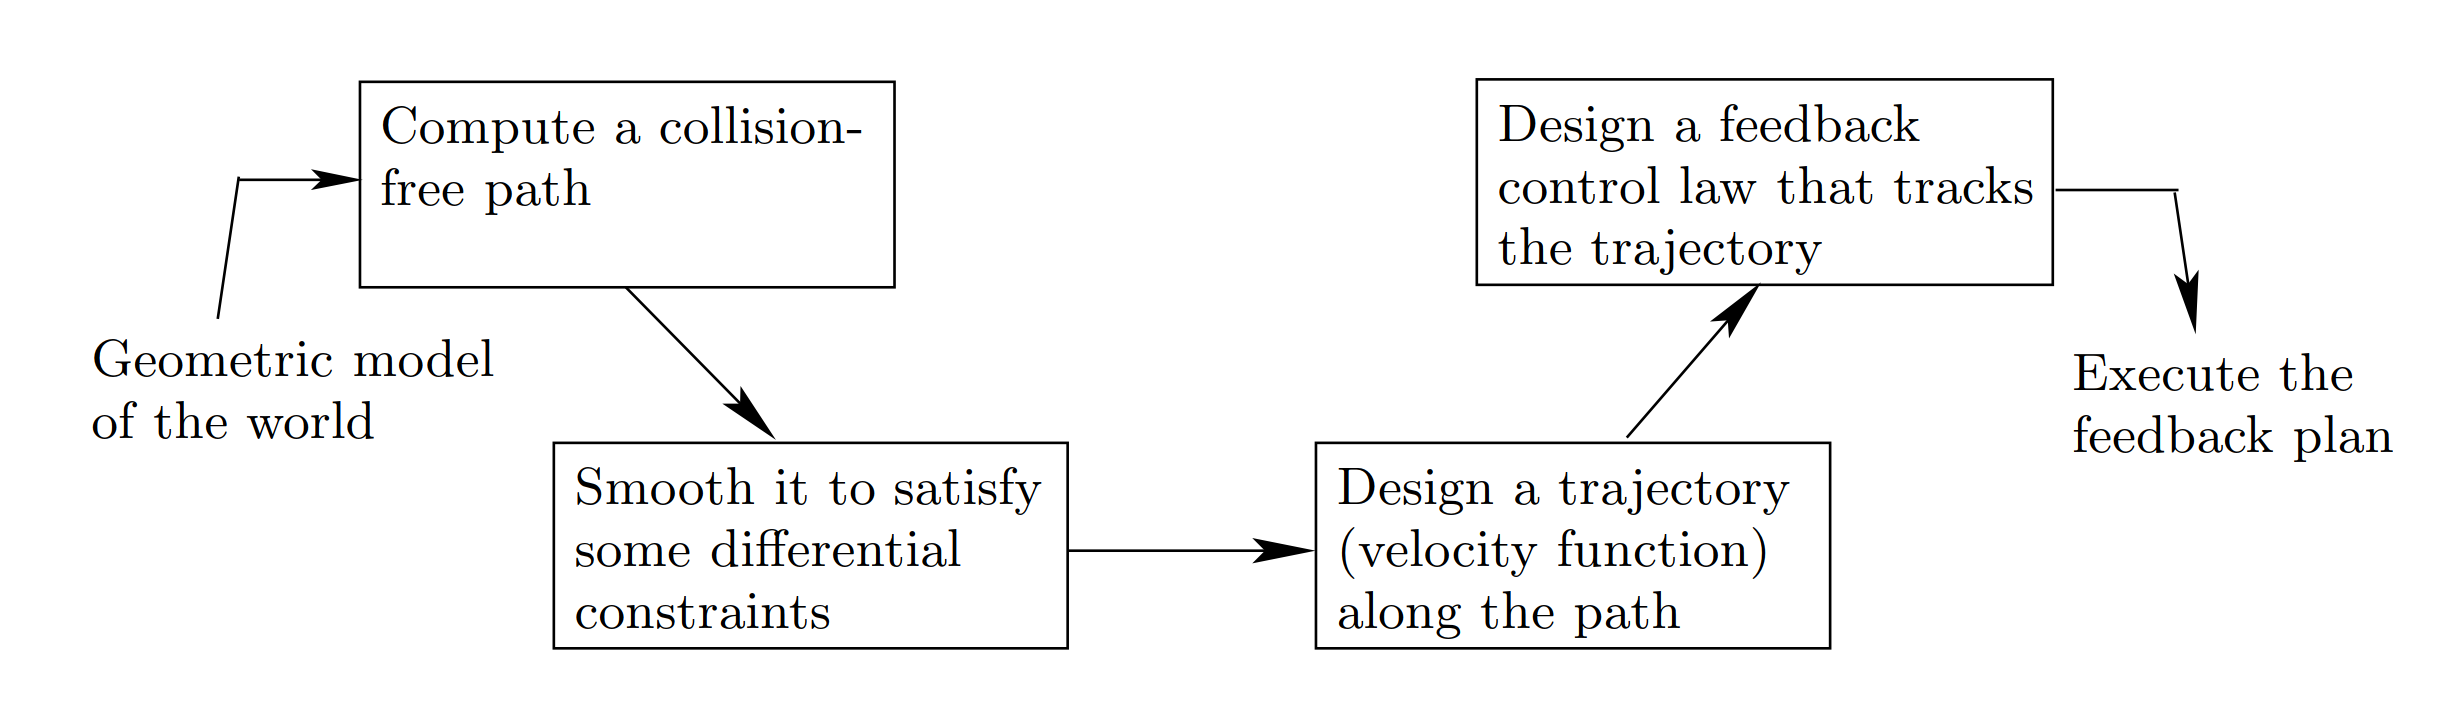
\includegraphics[width=6.5cm]{images/img247.png}
				\caption{Testbild in einem figure float} 
			\end{figure}
		\end{column}
	\end{columns}
\end{frame}
\begin{frame}{Graphen}{Sichtbarkeitsgraphen}
	\begin{columns}
		\begin{column}[T]{0.5\textwidth}
			\begin{itemize}
				\item Roadmap aus sichtbare Punkte bilden
				\item Die Eckpunkte der Hindernisse verbinden
				\item Sensoren nehmen neue Information für den Roboter, um neue  Kanten zu bilden
			\end{itemize}
		\end{column}
		\begin{column}[T]{0.5\textwidth}
			\begin{figure}
				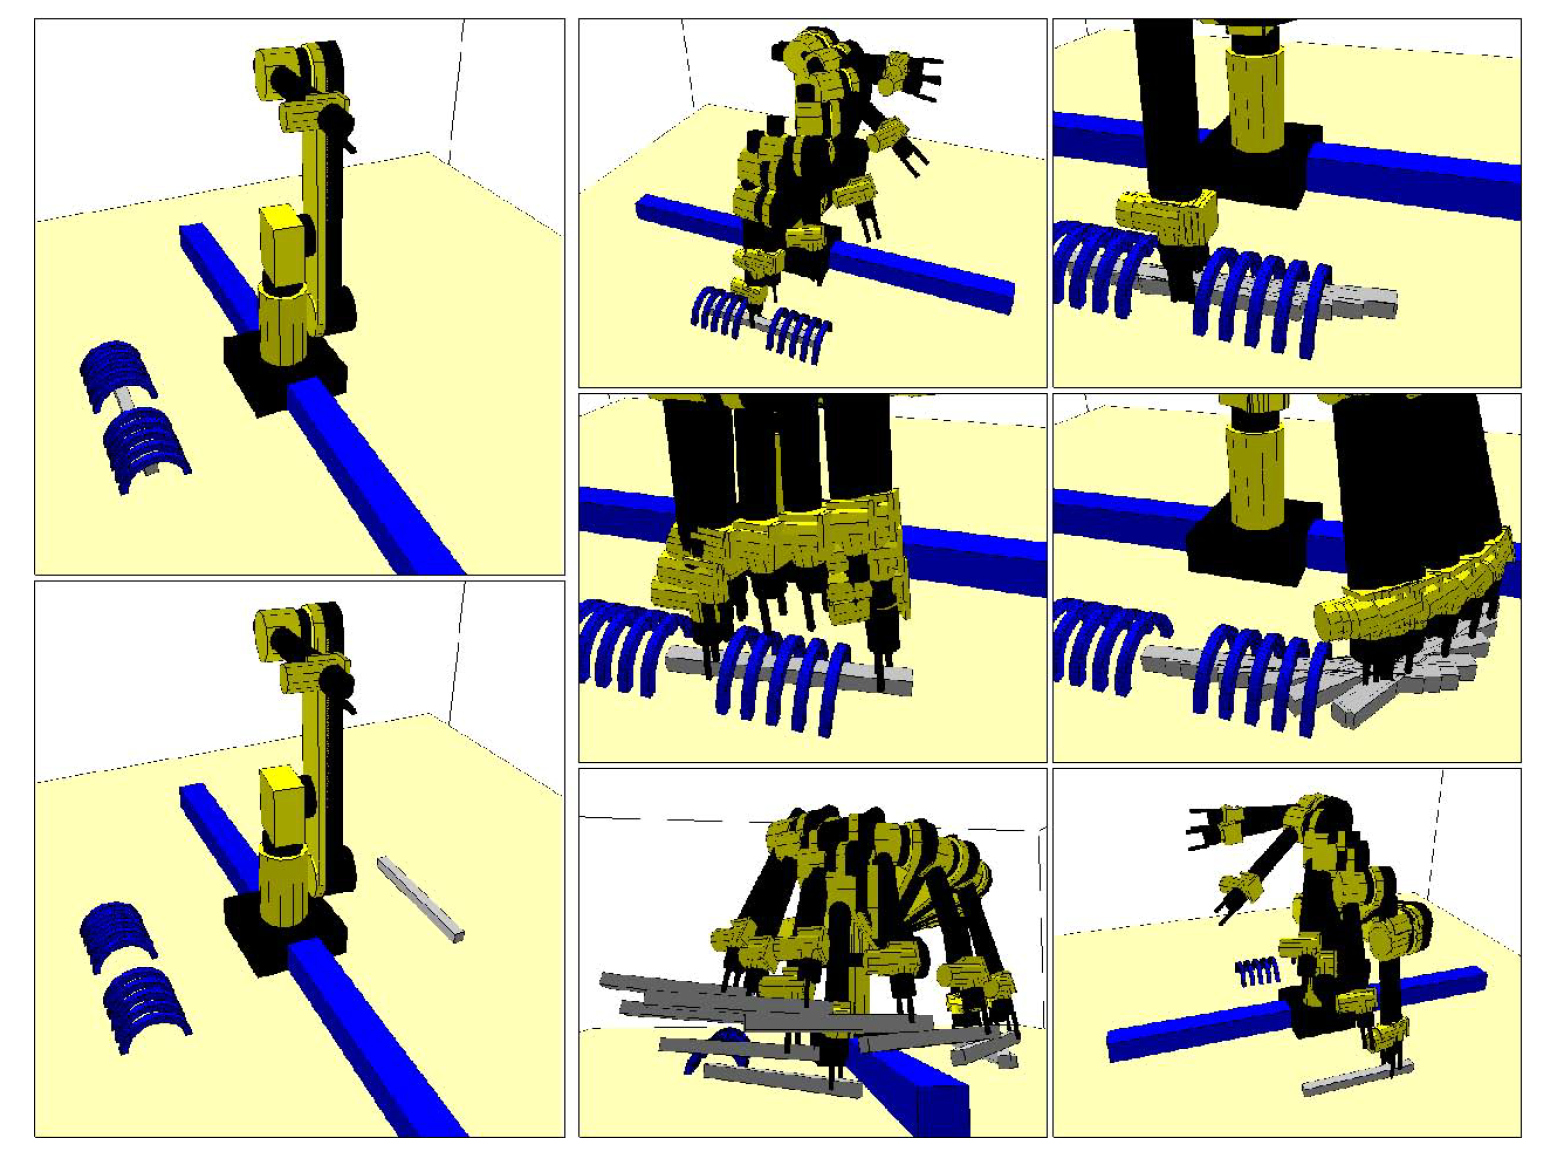
\includegraphics[width=6.5cm]{images/hierarchical.png}
				\caption{Testbild in einem figure float} 
			\end{figure}
		\end{column}
	\end{columns}
\end{frame}
\begin{frame}{Graphen}{Sichtbarkeitsgraphen}
	\begin{columns}
		\begin{column}[T]{0.5\textwidth}
			\begin{itemize}
				\item Roadmap aus sichtbare Punkte bilden
				\item Die Eckpunkte der Hindernisse verbinden
				\item Sensoren nehmen neue Information für den Roboter, um neue  Kanten zu bilden
			\end{itemize}
		\end{column}
		\begin{column}[T]{0.5\textwidth}
			\begin{figure}
				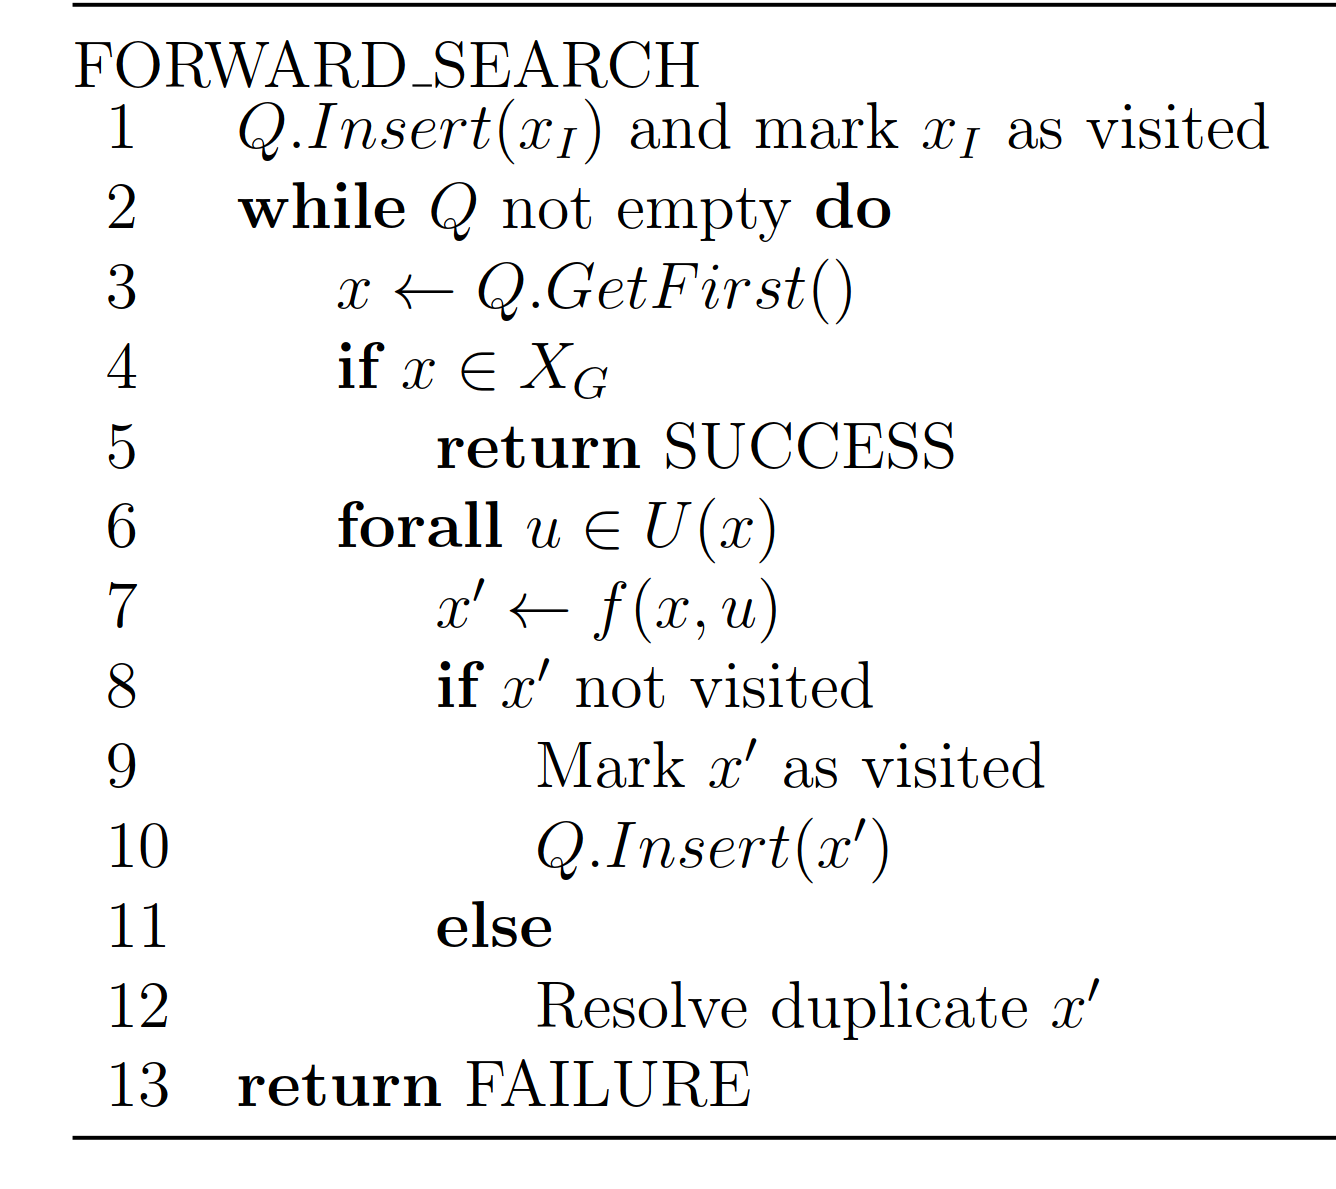
\includegraphics[width=6.5cm]{images/img225.png}
				\caption{Testbild in einem figure float} 
			\end{figure}
		\end{column}
	\end{columns}
\end{frame}

\section{tutorial}
\begin{frame}{Was ist Beamer?}{Eine Übersicht}
Das Beamer Paket für \LaTeX{} ermöglicht es, Präsentationsfolien zu erstellen und unterstützt dabei Features wie Animationen, die manuell nur mit viel Aufwand umgesetzt werden können.
Für die Details zu den Features siehe den Beamer User Guide\cite{BeamerDoc}.
\end{frame}

\begin{frame}
Folien in Beamer werden durch frame-Umgebungen definiert.
\end{frame}

\begin{frame}{Festlegen des Titels}{... und des Subtitels}
Die Frames verfügen über einen Titel und einen Subtitel.
Diese können entweder beim Öffnen der frame-Umgebung angegeben werden.
\end{frame}

\begin{frame}
	\frametitle{Festlegen des Titels}
	\framesubtitle{... und des Subtitels}
	Oder sie werden durch entsprechende Befehle angegeben.
\end{frame}

\begin{frame}{Strukturierung}{Aufzählungen}
\begin{itemize}
	\item Fließtext ist meistens nicht sinnvoll für Präsentationen
	\item Aufzählungen sind oft besser geeignet
	\begin{itemize}
		\item Geben Struktur
		\item Sorgen für Übersicht
	\end{itemize}
\end{itemize}
\begin{enumerate}
	\item Auf nummerierte Aufzählungen können verwendet werden
	\item Wie hier zu sehen ist
	\begin{enumerate}
		\item Auch mit
		\item Unterpunkten
	\end{enumerate} 
\end{enumerate}
\end{frame}

\begin{frame}{alert-Text}
	Wichtige Teile im Text können \alert<2>{durch alert hervorgehoben} werden.
	\begin{itemize}[<+-|alert@+>]
		\item Schritt 1
		\item Schritt 2
		\item Schritt 3
	\end{itemize}
\end{frame}

\subsection{Environments}
\begin{frame}{Environments}
\begin{theorem}
	Umgebungen wie theorem können auch in Beamer genutzt werden.
\end{theorem}
\begin{proof}
	Proof wird auch unterstützt.
\end{proof}
\begin{figure}
	
\includegraphics[width=3.5cm]{HochschuleLogo}
	\caption{Testbild in einem figure float}
\end{figure}
\begin{center}
	
\includegraphics[width=3.5cm]{HochschuleLogo}\\
	\emph{Testbild in center-Umgebung}
\end{center}
\end{frame}

\begin{frame}{Mathe-Modus}
	Der Mathe-Modus kann wie in LaTeX üblich benutzt werden:\\ 
	$\mathcal{F}: x = y + \frac{\mathsf{z}}{3}, y \in \mathbb{N}, \mathsf{z} \in \mathfrak{B}$ 
\end{frame}

\subsection{Blocks}
\begin{frame}{Blocks}
\begin{block}{Dies ist ein Block}
	Blocks können zur Strukturierung des Frame-Inhalts genutzt werden.
\end{block}
\begin{exampleblock}{Dies ist ein Beispielblock}
	Inhalt...
\end{exampleblock}
\begin{alertblock}{Dies ist ein Alert-Block}
	Inhalt...
\end{alertblock}
\end{frame}

\section{Anwendungen}



\begin{frame}[allowframebreaks]{allowframebreaks}
	Die Option allowframebreaks erlaubt es frames mit zu viel Inhalt umzubrechen. Dies ist besonders bei generiertem Inhalt wie dem Quellenverzeichnis sinnvoll.
	\\[1cm]
	\lipsum[1-2]
\end{frame}

\begin{frame}[fragile]{fragile}
\begin{lstlisting}
//Quellcode-Listings
//und andere Verbatim-Umgebungen
//setzen die fragile-Option des Frames voraus.
#include <iostream>
void main(){
	std::cout<<"Hallo Welt"<<std::endl;
}
\end{lstlisting}
\end{frame}

\section{Animationen}

\begin{frame}{Animieren mit Pause}
\begin{itemize}
	\item Schritt 1
	\item Schritt 2
	\pause
	\item Schritt 3
	\item Schritt 4
\end{itemize}
\end{frame}

\begin{frame}[<+->]{Ganzen Frame automatisch animieren}
	 %Das + steht immer fuer den naechsten Animationsschritt
\begin{itemize}
	\item Schritt 1
	\item Schritt 2
	\item Schritt 3
	\item Schritt 4
\end{itemize}
\end{frame}

\begin{frame}{Einzelne Umgebung automatisch animieren}
\begin{itemize}[<+->]
	\item Schritt 1
	\item Schritt 2
	\item Schritt 3
	\item Schritt 4
\end{itemize}
\end{frame}

\begin{frame}{Abweichende Animationsreihenfolge}{selbstdefiniert}
\begin{itemize}
	\item<1,3> Schritt 1
	\item<2-> Schritt 2
	\item<3-4> Schritt 3
	\item<5> Schritt 4
\end{itemize}
\end{frame}

\begin{frame}{Block-übergreifende Animation}{Übereinander}
\begin{block}{Bereich 1}
	\begin{itemize}
		\item<1-> Schritt 1
		\item<3-> Schritt 2
		\item<5-> Schritt 3
	\end{itemize}
\end{block}
\begin{block}{Bereich 2}
	\begin{itemize}
		\item<2-> Schritt 1
		\item<4-> Schritt 2
		\item<6-> Schritt 3
	\end{itemize}
\end{block}
\end{frame}
\note{Foliennotizen werden mit dem note-Befehl hinzugefügt.}

\begin{frame}{Block-übergreifende Animation}{Nebeneinander}
\begin{columns}[T]
\begin{column}[T]{0.5\textwidth}
\begin{block}{Bereich 1}
	\begin{itemize}
		\item<1-> Schritt 1
		\item<3-> Schritt 2
		\item<5-> Schritt 3
		\item<6-> Schritt 4
	\end{itemize}
\end{block}
\end{column}
\begin{column}[T]{0.5\textwidth}
\begin{block}{Bereich 2}
	\begin{itemize}
		\item<2-> Schritt 1
		\item<4-> Schritt 2
		\item<7-> Schritt 3
		\item<8-> Schritt 4
	\end{itemize}
\end{block}
\end{column}
\end{columns}
\end{frame}
\note{Diese Notizen werden nur ausgegeben, wenn die Option show notes gesetzt ist.}

\begin{frame}{Beliebige Inhalte ein- und ausblenden}
	\begin{itemize}[<+->]
		\item Schritt 1
		\item Schritt 2
		\item Schritt 3
		\item Schritt 4
	\end{itemize}
	\only<2>{Dieser Hinweis wird nur für Schritt 2 angezeigt.}
	\only<3>{Dieser Hinweis wird nur für Schritt 3 angezeigt.}
	Nachfolgender Text kann sich aber verschieben.
\end{frame}

\begin{frame}{Beliebige Inhalte ein- und ausblenden}
	\begin{itemize}[<+->]
		\item Schritt 1
		\item Schritt 2
		\item Schritt 3
		\item Schritt 4
	\end{itemize}
	\begin{overlayarea}{\textwidth}{1em}
		\only<2>{Dieser Hinweis wird nur für Schritt 2 angezeigt.}
		\only<3>{Dieser Hinweis wird nur für Schritt 3 angezeigt.}
	\end{overlayarea}
	Mit overlayarea verschiebt sich nachfolgender Text nicht.
\end{frame}

\begin{frame}{Beliebige Inhalte ein- und ausblenden}
	\begin{itemize}[<+->]
		\item Schritt 1
		\item Schritt 2
		\item Schritt 3
		\item Schritt 4
	\end{itemize}
	Inhalte können auch durch Animationen aufgedeckt werden.\\
	\uncover<2>{Dieser Hinweis wird nur für Schritt 2 angezeigt.}\\
	\uncover<3>{Dieser Hinweis wird nur für Schritt 3 angezeigt.}
\end{frame}

\section{Zeichnungen mit Animationen}
\begin{frame}{Animationen in Verbindung mit Zeichnungen}{Integration von Beamer mit tikz}
\begin{columns}[T]
	\begin{column}[T]{0.5\textwidth}
		\begin{center}
		\begin{tikzpicture}
			\useasboundingbox (-2,-2) rectangle (2,2);
			\node[draw,circle,fill=Senfgelb] (A) at (-1,0) {$A$}; 
			\node<3->[draw,circle,fill=Petrol,text=Senfgelb] (B) at ( 1,0) {$B$};
			\draw<5->[->] (A) to[out=45,in=135] (B);
			\draw<7->[->] (B) to[out=225,in=315] (A);			
		\end{tikzpicture}
		\end{center}
	\end{column}
	\begin{column}[T]{0.5\textwidth}
		\begin{itemize}
			\item Sei ein Knoten $A$ gegeben
			\item<2-> Wir fügen einen weiteren Knoten $B$ hinzu 
			\item<4-> Dann ziehen wir eine Kante von $A$ nach $B$
			\item<6-> ... und eine von $B$ nach $A$
		\end{itemize}
	\end{column}
\end{columns}	
\end{frame}

\section*{Schluss}
\begin{frame}
	\begin{center}
		\huge{Vielen Dank für die Aufmerksamkeit}
	\end{center}
	\begin{center}
		\Huge{Fragen?}
	\end{center}
\end{frame}

\begin{frame}[allowframebreaks]{\bibname}
\bibliography{tutorial}     %BibTeX-Datei literatur.bib
\end{frame}


\end{document}
